\chapter{Проектирование и разработка мобильного приложения на Anroid}

\section{Планирование и анализ рабочего процесса}

Диаграмма Ганта помогает распределить планируемое время по конкретным задачам. В данной работе составлена диаграмма Ганта, состаящая из 5 этапов, идущими последовательно. Представлена она на рисунке \ref{fig:гант} и составлена на период с 30 сентября 2024 года по 27 января 2025 года. 

\begin{figure}[h!]
\begin{center}
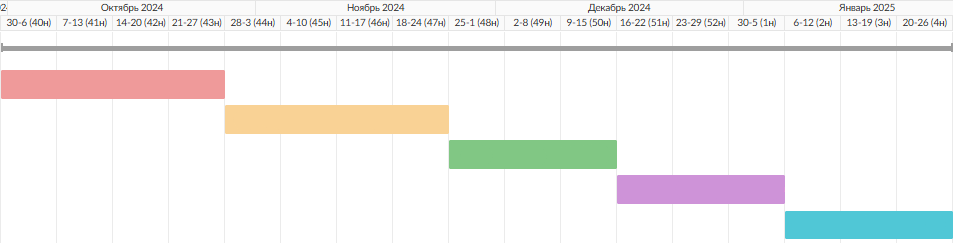
\includegraphics[width=1\hsize]{fig/гант.png}
\caption{Диаграмма Ганта}\label{fig:гант}
\end{center}
\end{figure}

На данной диаграмме красным цветом (первая строка) обозначена задача изучения предметной области (теоретических материалов). Желтым (вторая строка) -- формирование набора данных и обучение нейронной сети. Зеленым (третья строка) -- проектирование приложения и разработка серверной части. Фиолетовым цветом (четвертая строка) -- разработка интерфейса для мобильного приложения. Голубым (пятая строка) -- анализ полученных результатов, подведение итогов. 

По данной диаграмме больше всего времени планируется выделить на формирование набора данных (разметку, аннотирование и аугментацию изображений) и обучение нейронной сети, так как для качественного распознавания, нужно максимально точно разметить границы на каждом изображении. Кроме того, обучение нейросети, основанной на архитектуре YOLO с использованием аугментации, требует значительных временных и вычислительных ресурсов. Этап ознакомления с теоретическими материалы данной области также занимает много времени, поскольку, как описывалось в актуальности работы, аналогов такой программы пока не выпущено.

Каждой из задач требуется уделить особое внимание, поскольку все они могут повлиять на конечный результат. 

\section{Формирование набора данных, аннотирование и аугментация изображений}

Для создания качественного набора данных был проведен поиск изображений в открытых источниках, тематических группах и датасетах. Отбирались изображения с дефектами, описанными в первой главе. Найденные изображения загружались на платформу Roboflow в отдельный проект.

При подготовке данных особое внимание уделялось точной разметке изображений. Важно, чтобы границы дефектов соответствовали реальным размерам и не перекрывались. Если ограничивающая рамка больше реального дефекта, это может исказить представление о дефекте и затруднить обучение модели. Если рамки пересекаются, один и тот же дефект может быть отмечен несколькими рамками, что приводит к дублированию информации и искажению размеров. 

Данные ошибки снижают значение метрики Intersection over Union (пересечение над объединением -- показатель, характеризующий степень совпадения предсказанной рамки с истинной), что негативно сказывается на оценке качества обнаружения. Неточности в разметке могут привести к переобучению, когда модель становится чувствительной к шуму и не способна обобщать информацию на новые изображения.

На рисунках \ref{fig:big} и \ref{fig:Granitsi} продемонстрированы неправильно расставленные границы дефектов.

\begin{figure}[h!]
  \begin{minipage}[b]{0.45\hsize}
    \centering
    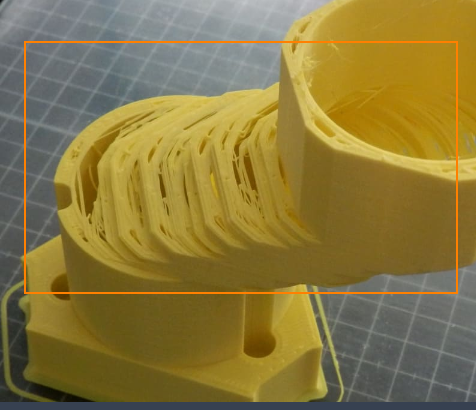
\includegraphics[width=\hsize]{fig/big.png}
    \caption{Слишком большие границы дефекта}
    \label{fig:big}
  \end{minipage}
  \hfill
  \begin{minipage}[b]{0.45\hsize}
    \centering
    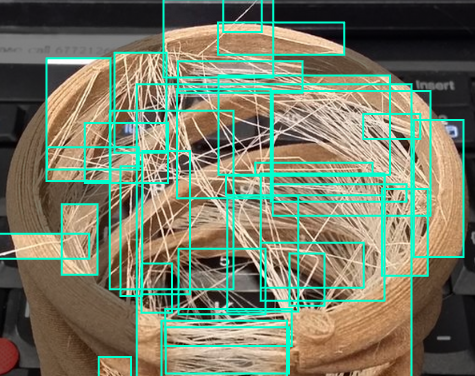
\includegraphics[width=\hsize]{fig/Granitsi.png}
    \caption{Границы дефектов перекрывают друг-друга}
    \label{fig:Granitsi}
  \end{minipage}
\end{figure}

Избегая данных ошибок при разметке, необходимо вручную разметить каждое изображение в наборе, выделяя дефекты разным цветом. Платформа Roboflow предлагает автоматическую разметку, но в данной задаче её точность оказалась недостаточной. Также Roboflow позволяет аннотировать изображения не только с помощью ограничивающих прямоугольников, но и полигонов, которые обеспечивают более точное описание контуров объектов. Изначально изображения были размечены с использованием полигонов, но их точность оказалась низкой, поэтому использовался классический вариант с прямоугольниками. Этот подход позволяет более стабильно и точно выделять дефекты, что является ключевым фактором для успешного обучения модели компьютерного зрения.

\section{Проектирование приложения и его серверной части}

Чтобы выполнять задачу обнаружения дефектов 3D-печати, требуются достаточно сложные вычислительные задачи. Чтобы снизить требования к Android-устройству было принято решение выполнять все вычисления и обработку изображений на серверной части. 

Централизованная серверная обработка обеспечивает безопасность и контроль качества, упрощает мониторинг и обновление моделей, а также снижает вероятность ошибок, связанных с разнообразием условий эксплуатации на конечных устройствах.

Серверная часть представляет собой веб-сервис, разработанный на языке Python с использованием микрофреймворка Flask (Flask --- фреймворк для создания веб-приложений на Python). Данный сервер предназначен для обработки изображений, получаемых через HTTP-запросы, и последующего обнаружения дефектов 3D-печати с использованием обученной модели, доступной через облачный API Roboflow.

Работа сервера начинается с инициализации приложения Flask, что позволяет ему принимать запросы от клиентов. Для обеспечения возможности взаимодействия с приложениями, работающими на других доменах или устройствах, используется библиотека flask cors (Cross-Origin Resource Sharing -- механизм, позволяющий осуществлять запросы с других источников).

После запуска сервера выполняется подключение к рабочему пространству и загрузка модели, обученной для обнаружения дефектов. Если модель не загружается корректно, сервер регистрирует ошибку, что позволяет избежать дальнейших сбоев при обработке запросов. Весь код серверной части представлен в приложении: Листинг \ref{ls:a:01}.

Основной функционал сервера реализован в эндпоинте (точке входа). Этот эндпоинт принимает POST-запросы, содержащие изображение и уникальный идентификатор устройства (device id). После проверки корректности полученного файла (например, формат файла должен быть JPG, JPEG или PNG) изображение сохраняется в папку uploads с уникальным именем, сформированным на основе device id и случайного уникального идентификатора (UUID -- Universally Unique Identifier, универсальный уникальный идентификатор).

После того как изображение было сохранено, сервер отправляет его в Roboflow для анализа с помощью метода predict, установив минимальный уровень доверия (confidence threshold) и параметр перекрытия (overlap). Минимальный уровень доверия представляет собой границу, ниже которой предсказанные объекты исключаются из рассмотрения. Это означает, что если модель не уверена в наличии дефекта с вероятностью выше установленного значения, то её предсказание не принимается во внимание. Такой подход позволяет уменьшить количество ошибочных срабатываний и повысить точность конечных результатов.

Параметр перекрытия определяет, насколько допустимо пересечение ограничивающих рамок различных предсказаний. Если эти рамки накладываются друг на друга на определённую величину, установленную параметром перекрытия, они могут быть объединены или одна из них может быть исключена как дублирующая. Такой подход позволяет более точно и однозначно выделить области, где были обнаружены дефекты.

Полученный результат содержит координаты ограничивающих рамок и метки обнаруженных дефектов. С использованием библиотеки OpenCV (Open Source Computer Vision Library -- библиотека для компьютерного зрения) изображение аннотируется: на него накладываются прямоугольники и текстовые метки, что визуально выделяет обнаруженные дефекты.

Аннотированное изображение сохраняется в папке «output». Сервер отправляет клиенту JSON-ответ, который включает в себя список обнаруженных дефектов и URL аннотированного изображения. 

Android-часть проекта -- клиентское приложение для обнаружения дефектов 3D-печати, разработанное с использованием языка программирования Kotlin и платформы Android. Архитектура приложения разделена на несколько ключевых компонентов, каждый из которых выполняет свою роль и обеспечивает взаимодействие с серверной частью для обработки изображений.

Файл MainActivity.kt -- это основа приложения. Он отвечает за первоначальную настройку интерфейса, проверку условий первого запуска, а также за скрытие панели управления, которая содержит элементы навигации. Кроме того, MainActivity.kt настраивает обработчики нажатий, позволяя пользователю легко перемещаться между экранами.

Файл OtherActivity.kt отвечает за выбор изображения и его предварительный просмотр. При помощи механизма выбора контента приложение получает URI выбранного изображения. Библиотека Glide (инструмент для быстрой загрузки и отображения изображений) используется для отображения выбранного изображения в интерфейсе. Дополнительно реализован процесс преобразования URI в локальный файл с использованием стандартных средств языка Java, что необходимо для дальнейшей передачи изображения на сервер.

Общение с серверной частью организовано с помощью RetrofitClient.kt, объекта, который настраивает клиент для выполнения HTTP-запросов посредством библиотеки Retrofit (фреймворк для работы с RESTful API -- интерфейс программирования приложений, основанный на архитектурном стиле REST). В конфигурации используется OkHttpClient (библиотека для работы с HTTP-запросами) с добавленным HttpLoggingInterceptor (инструмент для логирования HTTP-запросов), что позволяет отслеживать и отлаживать сетевую активность. Этот компонент устанавливает базовый URL сервера, задаёт таймауты соединения и чтения, а также создаёт экземпляр интерфейса ApiService.

Файл CustomHttpClient.java предоставляет дополнительные параметры настройки OkHttpClient, аналогичные тем, что используются в RetrofitClient.kt. Основное внимание уделяется расширенным настройкам таймаутов и логирования, что позволяет повысить стабильность и упростить отладку сетевых операций.

Интерфейс ApiService.kt описывает конечную точку API для загрузки изображения. С использованием аннотаций Retrofit (например, Multipart и POST) определяется тип запроса, позволяющий передавать изображение в формате multipart/form-data вместе с текстовым параметром, представляющим уникальный идентификатор устройства. 

При использовании данного формата тело запроса разбивается на несколько частей, каждая из которых отделена специальной строкой, называемой разделителем. Каждая часть запроса включает собственные заголовки, такие как Content-Disposition (заголовок, определяющий имя поля формы и, при необходимости, имя файла) и Content-Type (тип содержимого, например, image/jpeg для изображений). Благодаря этому можно передавать как текстовые параметры, так и файлы в одном запросе. Это обеспечивает корректную передачу данных на сервер, где изображение будет обработано и проанализировано для обнаружения дефектов.

Класс UploadResponse.kt представляет собой модель данных, которая включает в себя три важных поля: URL аннотированного изображения, список обнаруженных дефектов (classes) и идентификатор устройства (device id). Эти данные возвращаются сервером и используются в приложении для отображения результатов обработки.

\section{Интерфейс разработанного приложения для обнаружения дефектов 3D-печати}

Интерфейс приложения должен быть спроектирован таким образом, чтобы обеспечить пользователю комфортное взаимодействие с функциональными возможностями системы. В процессе проектирования интерфейса были применены принципы минимализма, интуитивной навигации и визуального оформления, что способствует повышению удобства использования приложения.

Цветовая гамма представляет собой один из главных аспектов дизайна пользовательского интерфейса, оказывая значительное влияние на восприятие приложения, его эстетическую привлекательность и удобство использования.

В процессе разработки интерфейса мобильного приложения были выбраны следующие цветовые решения: тёмно-зелёный цвет для фона, белый -- для акцентов и текста, а также светло-зелёный -- для второстепенных элементов.

Такое цветовое решение обеспечивает удобство использования приложения, способствует повышению читаемости и создаёт впечатление профессионализма и технологичности продукта. Эти аспекты играют ключевую роль в достижении основной цели разработки.

Логотип приложения должен отображать его суть, поэтому за основу взят зигзагообразный рисунок, который используется в 3D-печати для создания дна и крыши деталей. Чтобы отразить связь с анализом и машинным зрением, в центре логотипа расположена камера, напоминающая о цели приложения. Созданный на основе выбранных цветов логотип продемонстрирован на рисунке \ref{fig:logo}.

\begin{figure}[h!]
\begin{center}

\includegraphics[width=0.4\hsize]{fig/logo.png}
\caption{Логотип разработанного приложения}\label{fig:logo}
\end{center}
\end{figure}

При первом запуске приложения пользователь оказывается на приветственной странице, где представлена вся необходимая информация о приложении и инструкции по загрузке фотографии детали для анализа. 

Одним из ключевых требований к загружаемому изображению является его чёткость и фокусировка на детали. Для этого важно держать телефон неподвижно, чтобы дефект на детали был в центре кадра. Использование однотонного фона значительно упрощает обнаружение дефектов, так как объекты на фоне не будут ошибочно приняты за дефекты.

Освещение должно быть тщательно подобрано таким образом, чтобы исключить появление теней на объекте, но при этом избежать его пересвечивания, поскольку это может затруднить распознавание.

Рядом с каждым пунктом рекомендаций находится кнопка, которая открывает подробное описание требований. Это позволяет пользователю лучше понять, что именно нужно сделать для получения качественного результата.

Некоторые фрагменты текста выделены скруглёнными бледно-зелёными блоками, что придаёт им визуальную выразительность и помогает выделить их на общем фоне. Кнопки, выполненные в белых блоках, делают их более интуитивно понятными и удобными для использования.

На странице загрузки фотографии после нажатия на кнопку выбора открывается стандартное окно выбора фотографий на Android. Здесь можно либо сделать новую фотографию, либо выбрать уже сделанную ранее. Отдельной кнопкой можно отправить фотографию на сервер. После получения ответа исходное изображение заменяется на аннотированное, а ниже списком отображаются все обнаруженные дефекты. При необходимости пользователь может открыть страницу с подробным описанием дефекта, включая его характерные особенности, причины возникновения и рекомендации по устранению. Это позволяет понять проблему и предотвратить её повторение.

Благодаря последовательному процессу взаимодействия с приложением пользователь может быстро загрузить фотографию детали, отправить её на анализ и получить точные результаты. Интуитивно понятный интерфейс и пошаговая структура минимизируют вероятность ошибок, делая приложение удобным даже для новичков. На рисунках \ref{fig:obuchenie} и \ref{fig:1} продемонстрирована приветственная страница и страница загрузки фотографии.

\begin{figure}[h!]
  \begin{minipage}[b]{0.45\hsize}
    \centering
    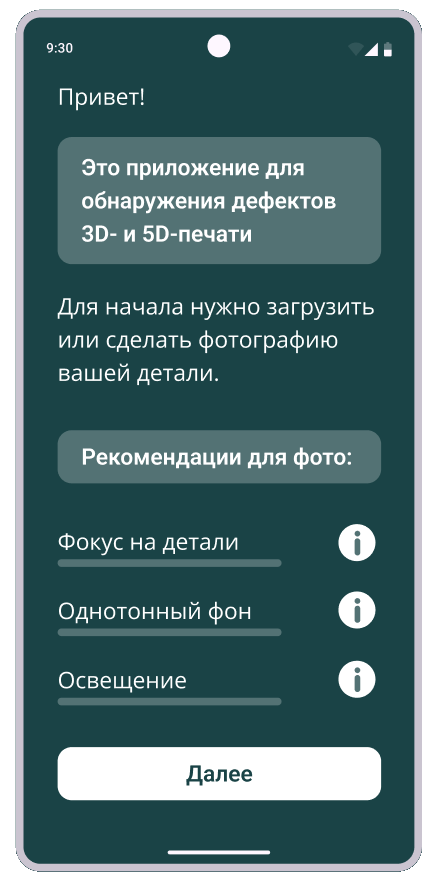
\includegraphics[width=\hsize]{fig/1.png}
    \caption{Приветственная страница с рекомендациями}
    \label{fig:obuchenie}
  \end{minipage}
  \hfill
  \begin{minipage}[b]{0.45\hsize}
    \centering
    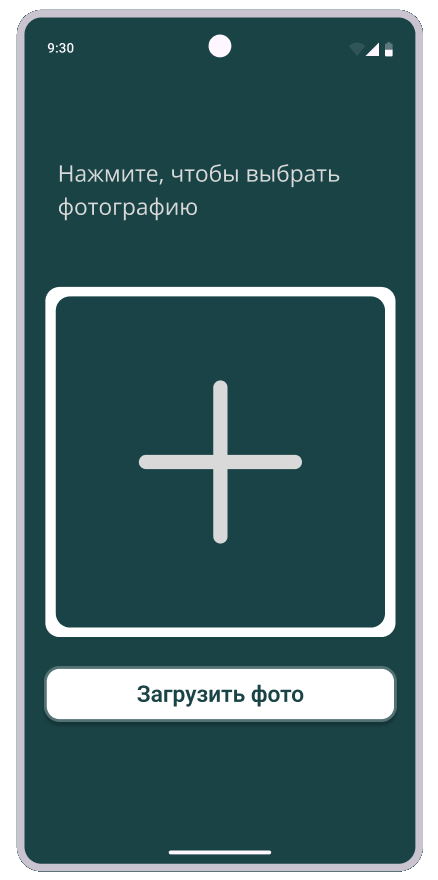
\includegraphics[width=\hsize]{fig/2.png}
    \caption{Страница загрузки фотографии}
    \label{fig:1}
  \end{minipage}
\end{figure}


\section{Обнаруженные недостатки выбранного подхода к распознаванию дефектов}

Изначально модель обучалась на 6 классах~-- это «спагетти», «паутина», деламинация, искревление геометрии, недоэкструзия и перегрев. Во время проведения поиска изображения для обучения нейросети возникла проблема, что в открытом доступе количество данных для одних классов значительно больше, чем для других. Например, найти качественные изображения с дефектом «спагетти» оказалось намного проще, чем для перегрева. После этапа формирования датасета получилось следующее соотношение: 1 класс~-- «спагетти»~-- 35~\%, 2 класс~-- «паутина» -- 20~\%, 3 класс~-- деламинация -- 10~\%, 4 класс~-- недоэкструзия~-- 15~\%, 5 класс~-- искревление геометрии~-- 10\%, 6 класс~-- перегрев~-- 10~\%. Процентное соотношение является приблизительным, поскольку в процессе создания аннотаций некоторые изображения были исключены.
График соотношения размеров классов от общего числа изображений представлен на рисунке \ref{fig:123456}.

\begin{figure}[h!]
\begin{center}
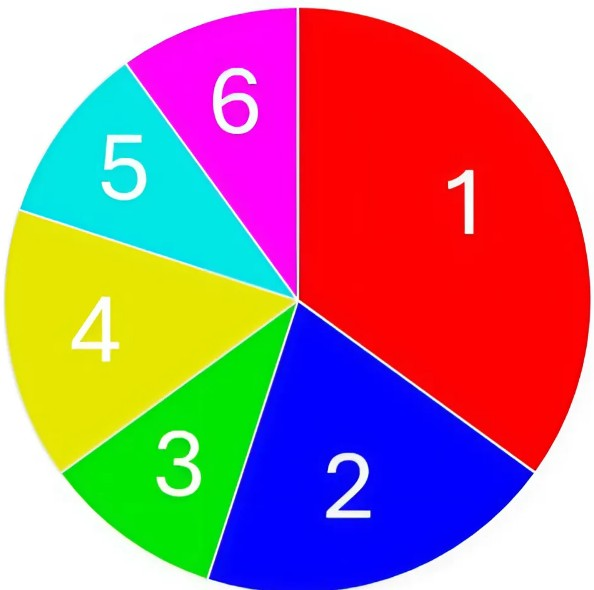
\includegraphics[width=0.4\hsize]{fig/123456.jpeg}
\caption{График соотношения размеров классов от общего числа изобра
жений}\label{fig:123456}
\end{center}
\end{figure}

Равномерное распределение классов в наборе данных критически важно для корректного обучения нейросети, поскольку дисбаланс может привести к значительному снижению точности предсказаний.

По графику заметно, что класс «спагетти» является самым большим, но это обусловлено тем, что дополнительным фактором, влияющим на размер класса, является его высокая вариативность. В отличие от других типов дефектов, «спагетти» может иметь широкий спектр визуальных проявлений: от единичных вытянутых нитей до плотных скоплений спутанного материала. Эта особенность усложняет процесс классификации, поскольку для эффективного распознавания необходимо учесть множество возможных конфигураций дефекта.

С другой стороны, класс делеминации составляет всего лишь 10~\% от общего объема изображений, но этого хватило для того, чтобы научить нейросеть достаточно хорошо находить этот дефект. Проблема возникает в том, что добиться того, чтобы нейросеть отличала делеминацию от недоэкструзии, так и не получилось.

Сложность в разграничении этих классов заключается в том, что оба дефекта могут проявляться визуально схожим образом. 

Особенно сложной ситуация становится в случае, когда недоэкструзия развивается горизонтально относительно стола 3D-принтера. Деламинация представляет собой расслоение, возникающее из-за недостаточной адгезии между слоями. Визуально это выражается в наличии разрывов или отслоений, расположенных горизонтально. Недоэкструзия же связана с нехваткой подаваемого материала, что приводит к появлению участков с уменьшенной толщиной слоя или разрывами в структуре. При вертикальном проявлении недоэкструзия выглядит как истончение стенок или неравномерное наполнение, что делает ее относительно легко отличимой. Однако при горизонтальной недоэкструзии, когда слой формируется с недостаточным количеством материала, он может напоминать деламинацию по внешнему виду, создавая разрывы, схожие с отслоением.

Исходя из этой проблемы, было решено на данном этапе оставить только дефект деламенации. Исключение недоэкструзии из набора позволило увеличить точность обнаружения деламенации. В дальнейшем возможно повторное введение класса «недоэкструзия».

На рисунках \ref{fig:nedo} и \ref{fig:delam} продемонстрирована схожесть дефектов недоэкструзии и деламенации, что увеличивает ошибку
\begin{figure}[h!]
  \begin{minipage}[b]{0.45\hsize}
    \centering
    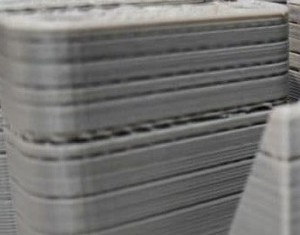
\includegraphics[width=\hsize]{fig/nedo.jpg}
    \caption{Дефект недоэкструзии на детали}
    \label{fig:nedo}
  \end{minipage}
  \hfill
  \begin{minipage}[b]{0.45\hsize}
    \centering
    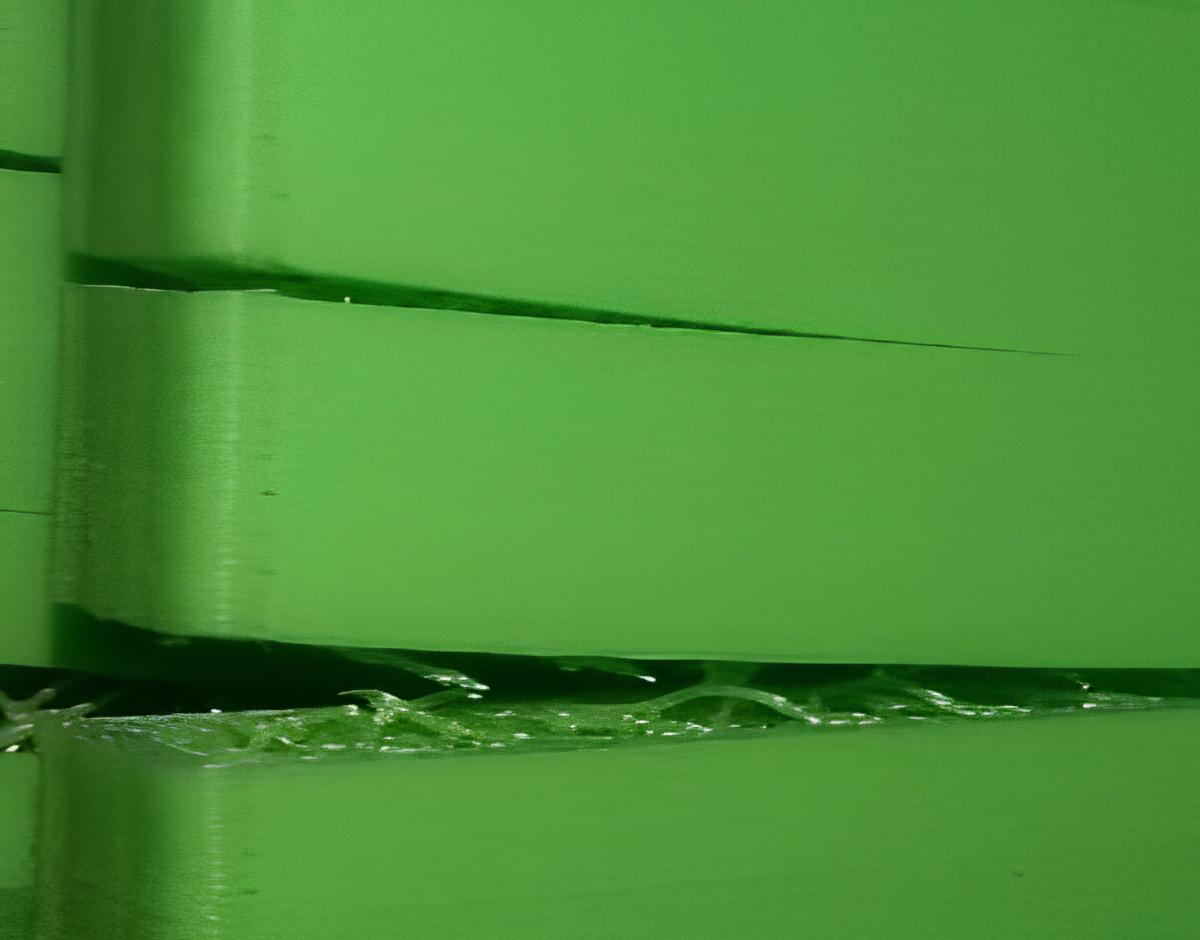
\includegraphics[width=\hsize]{fig/delam.jpg}
    \caption{Дефект деламенации на детали}
    \label{fig:delam}
  \end{minipage}
\end{figure}

Класс с дефектом перегрева, также пришлось удалить из набора из-за недостаточного количества и качества обучающих материалов. В конечном итоге осталось 4 класса.

Оценка точности работы нейросети требует использования специальных метрик, которые позволяют измерить качество предсказаний. Для объективной оценки используется показатель средней точности по классам при пороговом значении 0.5 (Average Precision by Class at IoU 0.5), сокращенно mAP50.

Данный показатель основан на метрике пересечения по объединению (Intersection over Union, IoU), которая измеряет степень совпадения предсказанной области с реальной. Если значение IoU превышает 0.5 (то есть пересечение составляет не менее 50~\% от общей площади двух областей), предсказание считается успешным.

Средняя точность (AP, Average Precision) рассчитывается для каждого класса отдельно и определяется как площадь под кривой, построенной по зависимости между точностью (Precision~-- доля корректных предсказаний среди всех найденных объектов) и полнотой (Recall~-- доля правильно найденных объектов среди всех существующих в данных).

Средняя средняя точность (mAP, Mean Average Precision)~-- это усредненное значение AP по всем классам. Показатель mAP50 учитывает только предсказания с IoU~$\geq$ 0.5 и используется в качестве базового критерия для оценки качества детекции. Чем выше его значение, тем точнее модель распознает дефекты, не требуя при этом строгого совпадения предсказанных и реальных границ.

Таким образом, точность по классам следующая: «спагетти»~-- 48~\%, «паутина»~-- 28~\%, деламинация~-- 31~\%, искревление геометрии~-- 31~\%.

Графики динамики ключевых метрик в процессе обучения нейросети представлены в приложении \ref{fig:1results} и \ref{fig:2results}. На всех графиках по оси X отложены итерации (эпохи) обучения, что показывает, как изменяются метрики со временем. По оси Y — значения соответствующих метрик: потерь, точности, полноты и средней точности.

Синяя линия — реальные измеренные значения метрик на каждой итерации обучения. Она имеет значительные колебания, так как значения метрик могут изменяться от набора данных, на каждом шаге.

Красная пунктирная линия~-- сглаженный тренд этих значений, который показывает общую тенденцию изменения метрик и помогает лучше понять, как модель обучается в целом.

Потери на классификации (class loss)~--  насколько хорошо модель различает классы. В начале обучения потери высокие, но со временем снижаются. Модель постепенно обучается правильно определять классы дефектов.

Потери на определении границ объектов (box loss)~-- точность определения границ дефектов. Видно, что этот показатель имеет тенденцию к росту, что говорит о проблемах с определениями границ дефектов.

Потери на обнаружении объектов (obj loss)~-- отражает, насколько хорошо модель определяет наличие дефекта. По графику виден рост, но колебания указывают на нестабильность.

Точность предсказаний (precision)~-- показывает долю правильно предсказанных дефектов среди всех обнаруженных. Значение постепенно увеличивается, значит точность растет.

Полнота предсказаний (recall)~-- измеряет, насколько полно модель находит дефекты. В начале обучения значение низкое, но затем постепенно увеличивается, что указывает на улучшение способности модели находить все дефекты в изображениях.

Средняя точность по классам при IoU~$\geq$ 0.5 (mAP)~-- характеризует общий уровень точности модели при небольших отклонениях в границах.

Средняя точность по классам при IoU от 0.5 до 0.95 (mAP 50 95)~-- показывает среднее значение точности модели по всем классам при разных значениях порога пересечения по объединению. Его значения остаются значительно ниже, чем у mAP50, что говорит о том, что при высоких значениях IoU модель испытывает трудности с точным определением границ дефектов.

Графики показывают, что модель постепенно обучается, ошибки классификации снижаются, точность и полнота предсказаний растут, но потери при обнаружении объектов и границ указывают на проблемы. Разница между mAP50 и mAP5095 говорит о том, что модель пока неточно определяет границы дефектов.

\section{Результат разработки и возможные методы улучшения работы приложения}

В результате работы удалось распознать четыре вида дефектов. Основной трудностью было различие между дефектами деламинации и недоэкструзии. Несмотря на аннотирование данных, нейросеть продолжала путать эти типы дефектов, особенно при горизонтальном проявлении недоэкструзии. Для повышения точности распознавания было решено временно исключить класс недоэкструзии из набора данных.

При тестировании приложения были обнаружены проблемы с обработкой малоразмерных изображений на серверной части. Для решения проблемы было внедрено автоматическое увеличение изображений до минимального рабочего разрешения в 800 на 800 пикселей. Результат обработки изображения и вывод списка дефектов представлен на рисунке \ref{fig:find}.

\begin{figure}[h!]
\begin{center}
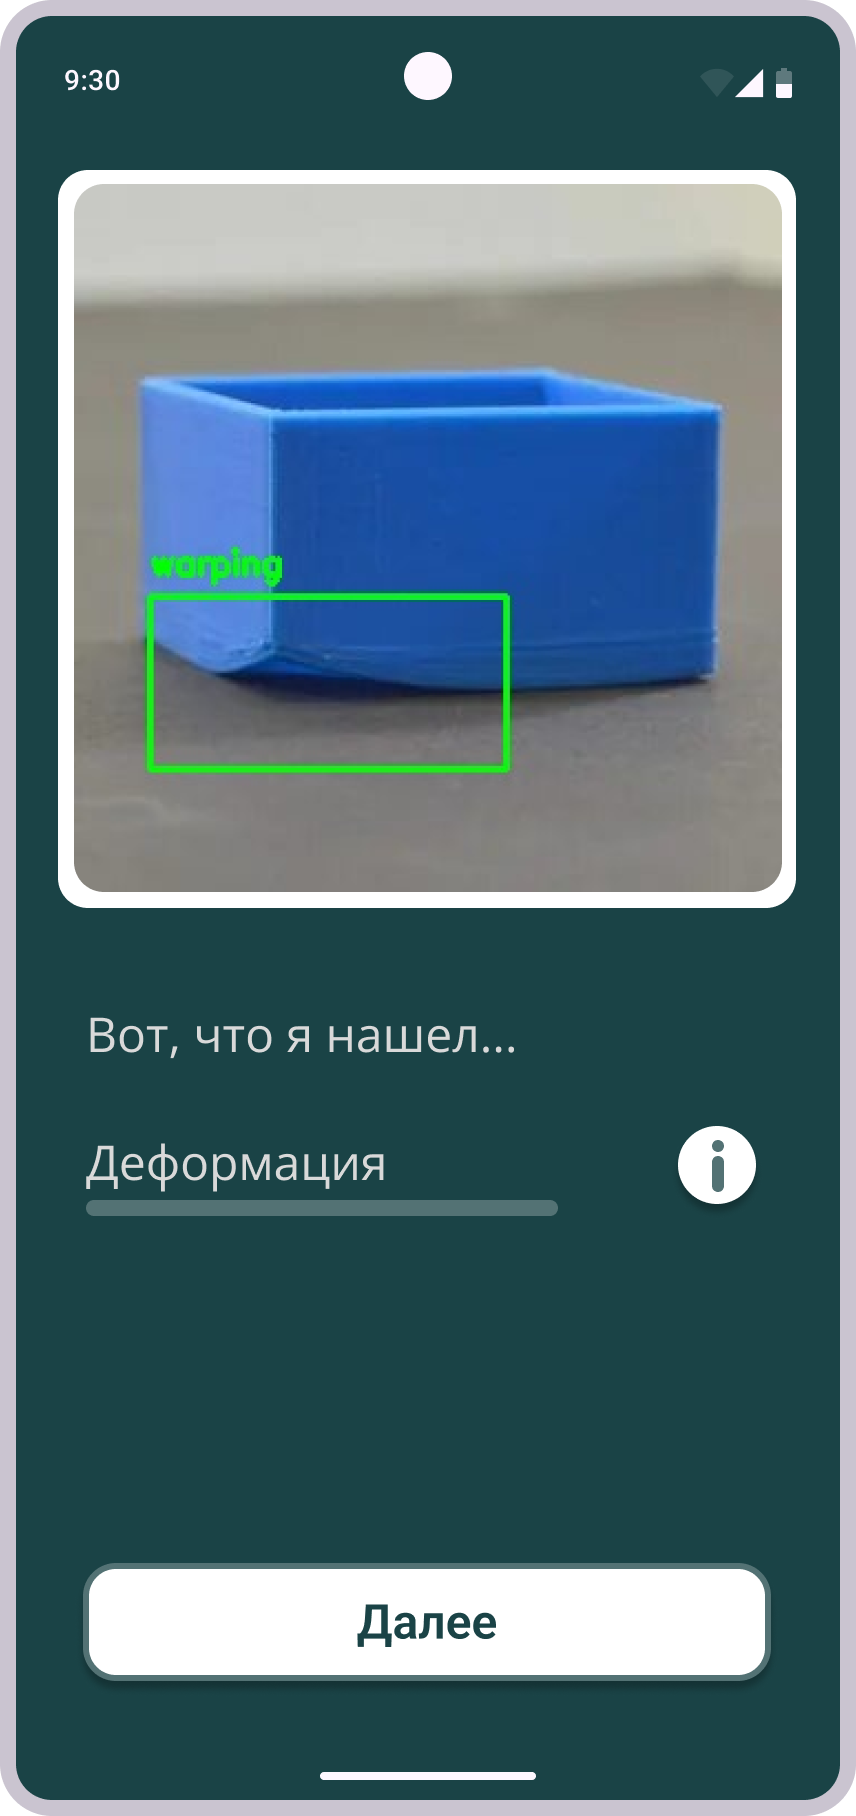
\includegraphics[width=0.4\hsize]{fig/find.png}
\caption{Экран с найденными ошибками и аннотированным изображением}\label{fig:find}
\end{center}
\end{figure}

Для тестирования качества распознавания дефектов были загружены изображения разной степени сложности. Анализируя полученные результаты распознавания дефектов, можно прийти к выводу, что даже на изображениях низкого качества нейросеть способна обнаружить дефекты с такой же точностью, как и на более чётком ее варианте, что означает эффективность проведенной аугментации.

Одна из главных проблем задачи заключается в том, что нейросети не всегда удается интерпритировать геометрию обьекта, чтобы определить на нем дефект. Часто явный дефект деламинации не распознавался из-за того, что на изображении была видна внутренняя геометрия объекта. Из-за этого нейронная сеть не могла с достаточной точностью определить его тип.
Подобная проблема представлена в приложении на рисунке \ref{fig:HeCracking} и \ref{fig:cracking}.

Изначально модель обучалась на 6 классах~-- это «спагетти», «паутина», деламинация, искревление геометрии, недоэкструзия и перегрев. Эти недостатки являются одними из самых визуально отличимых в 3D-печати, что должно было значительно облегчить процесс обучения, но из-за сложной геометрии фигур и их многообразия задача оказалась довольно сложной и трудоёмкой. Модель была обучена на части этих классах и теперь способна обнаруживать аналогичные дефекты. Планируется расширить список классов, включив другие виды дефектов 3D-печати, чтобы повысить точность распознавания и эффективность модели.

Эту ситуацию может улучшить внедрение единой тестовой модели, призванной выявить как можно больше дефектов. Такой подход способен значительно повысить точность обнаружения, поскольку процесс обучения будет происходить не только на различных деталях, но и на этой тестовой модели. Подобные модели находятся в открытом доступе, что значительно облегчает процесс создания единой детали для выявления дефектов. В дополнение к этому, планируется внедрение специальных маяков, которые должны помочь нейросети более точно понимать, как и с какого ракурса была сделана фотография. Это может улучшить качество анализа и ускорить процесс выявления дефектов. Подобная модель представлена на рисунке \ref{fig:test}.

\begin{figure}[h!]
\begin{center}
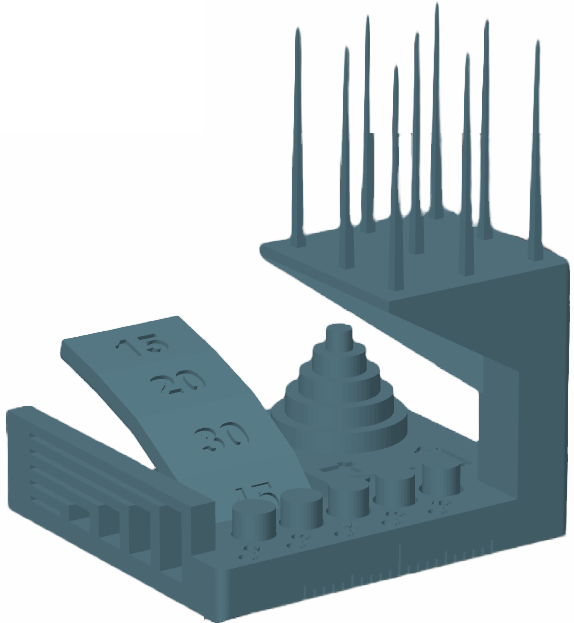
\includegraphics[width=0.55\hsize]{fig/Test.png}
\caption{Пример единой модели, печатаемой для выявления дефектов}\label{fig:test}
\end{center}
\end{figure}
